%! TEX program = pdflatex
\documentclass{beamer}

\usepackage[utf8]{inputenc}
\usepackage{utopia}            % font utopia imported
\usepackage{amsmath}
\usepackage{latexsym}
\usepackage{calc}              % support command '\widthof'
\usepackage{xcolor}            % support multiple color 
\usepackage{arydshln}
\usepackage{amssymb}  
\usepackage{booktabs}
\usepackage{graphicx}
\usepackage{subcaption}
\usepackage{bookmark}
\usepackage{float}

\usefonttheme{professionalfonts} % using non standard fonts for beamer
%\usefonttheme{serif} % default family is serif
%\usepackage{fontspec}
%\setmainfont{Liberation Serif} 

\makeatletter
\let\@@magyar@captionfix\relax
\makeatother

\usetheme{Madrid}
\usecolortheme{default} 

%%%%%%%%%%%%%%%%%%%%%%%%%%%%%%%%%%%%%%%%%%%%%%%%%%%%%%%%%%%%%%%%%%
\title[CMT.Tsinghua]{Wannier Functions}

\subtitle{(Technique Details of \emph{Wannier90})}

\author[Yang Li]
{Yang Li\inst{1}}  

\institute[Physics@Tsinghua] 
{
  \inst{1}%
  Department of Physics\\
  Tsinghua University 
}

\date[Tsinghua Physics 2019]{Jan 2019}
%%%%%%%%%%%%%%%%%%%%%%%%%%%%%%%%%%%%%%%%%%%%%%%%%%%%%%%%%%%%%%%%%

%%%%%%%%%%%%%%%%%%%%%%%%%%%%%%%%%%%%%%%%%%%%%%%%%%%%%%%%%%%%%%%%%
\AtBeginSection[]
{
  \begin{frame}
    \frametitle{Table of Contents}
    \tableofcontents[currentsection]
  \end{frame} 
}
%%%%%%%%%%%%%%%%%%%%%%%%%%%%%%%%%%%%%%%%%%%%%%%%%%%%%%%%%%%%%%%%%
 
\begin{document}
  %%%%%%%%%%%%%%%%%%%%%%%%%%%%%%%%%%%%%%%%%%%%%%%%%%%%%%%%%%%%%%%%%
  \frame{\titlepage}
  %%%%%%%%%%%%%%%%%%%%%%%%%%%%%%%%%%%%%%%%%%%%%%%%%%%%%%%%%%%%%%%%%

  %%%%%%%%%%%%%%%%%%%%%%%%%%%%%%%%%%%%%%%%%%%%%%%%%%%%%%%%%%%%%%%%%
  \begin{frame}
    \frametitle{Table of Contents}
    \tableofcontents
  \end{frame}
  %%%%%%%%%%%%%%%%%%%%%%%%%%%%%%%%%%%%%%%%%%%%%%%%%%%%%%%%%%%%%%%%%
  
  \section{Bolch Theorem}

  %%%%%%%%%%%%%%%%%%%%%%%%%%%%%%%%%%%%%%%%%%%%%%%%%%%%%%%%%%%%%%%%%
  \begin{frame}
    \frametitle{Defination of \(\widehat{T}_l\)}
    For crystal system, the Hamiltonlian is commutes with the translation operators \(\widehat{T}_l\).
    \begin{equation}
      \left[\widehat{T_l},\widehat{H}\right] = 0
    \end{equation}

    Where  \textcolor{purple}{\(\widehat{H} = \widehat{T} + \widehat{V}(\mathbf{r})\),} \(\widehat{V}(\mathbf{r}) = \widehat{V}(\mathbf{r}+\mathbf{R}_l)\), \textcolor{purple}{\(\widehat{T}_l|\psi(\mathbf{r})\rangle = |\psi(\mathbf{r}+\mathbf{R}_l)\rangle\),} \(\mathbf{R}_l = \sum_{i=1}^3l_i\mathbf{a}_i\), \textcolor{purple}{and \{\(\mathbf{a}_i\)\} is the lattice vector}.
     
    \begin{block}{Properties}
      \begin{displaymath} 
        \left. \begin{array}{r}
          \widehat{T}_l\widehat{T}_{l'} = \widehat{T}_{l+l'}\\
          \widehat{T}_l|\psi({\mathbf{r})}\rangle = t_l|\psi({\mathbf{r})}\rangle
        \end{array}  \right\} \Rightarrow t_{l+l'} = t_l\cdot{}t_{l'}
      \end{displaymath}
    \end{block}

    The eigenvalue of \(\widehat{T}_l\) can be writen as: 
    \begin{equation}
      t_l = \left(t_{\mathbf{a}_1}\right)^{l_1}\left(t_{\mathbf{a}_2}\right)^{l_2}\left(t_{\mathbf{a}_3}\right)^{l_3}
    \end{equation}  

  \end{frame}
  %%%%%%%%%%%%%%%%%%%%%%%%%%%%%%%%%%%%%%%%%%%%%%%%%%%%%%%%%%%%%%%%% 

  %%%%%%%%%%%%%%%%%%%%%%%%%%%%%%%%%%%%%%%%%%%%%%%%%%%%%%%%%%%%%%%%%
  \begin{frame}
  \frametitle{Eigenvalue of \(\widehat{T}_l\)}
  
  Let \(\widehat{T}(\mathbf{a}_i) |\psi(\mathbf{r})\rangle = |\psi(\mathbf{r}+l_i\mathbf{a}_i)\rangle\). The translation operator \(\widehat{T}(\mathbf{a}_i)\) generate a cyclic group \(C_{N_i}\) in the real space\textcolor{gray}{, where \(N_i\) is the cell quantity in \(\mathbf{a}_i\) direction among one period of total wave functions}.

  \begin{block}{Noting}
    Since the \(C_{N_i}\) is also a finite ablian group, accroding to \emph{Schur's Lemma I}, all of its \textcolor{purple}{inreducable unitary representation} is \textcolor{purple}{one dimensional}, which means, \(t(\mathbf{a}_i) = \mathrm{e}^{\mathrm{i}2\pi{}y_i}\)
  \end{block}

  Using the periodic conditions: \(t(\mathbf{a}_i)^{N_i}=1\), one can easily conclude that, 
  \begin{subequations}
    \begin{align}
      t(\mathbf{a}_i) &= \mathrm{e}^{\mathrm{i}2\pi{}\frac{m_i}{N_i}}\\
      t_l &= \mathrm{e}^{\mathrm{i}2\pi{}\left(\frac{m_1l_1}{N_i}+\frac{m_2l_2}{N_2}+\frac{m_3l_3}{N_3}\right)}
    \end{align}
  \end{subequations}

  If we set \(\mathbf{k} = \frac{m_1}{N_1}\mathbf{b}_1+\frac{m_2}{N_2}\mathbf{b}_2+\frac{m_3}{N_3}\mathbf{b}_3\), and \(\mathbf{a}_i\cdot\mathbf{b}_j = 2\pi\delta_{ij}\)

  \end{frame}
  %%%%%%%%%%%%%%%%%%%%%%%%%%%%%%%%%%%%%%%%%%%%%%%%%%%%%%%%%%%%%%%%% 

  %%%%%%%%%%%%%%%%%%%%%%%%%%%%%%%%%%%%%%%%%%%%%%%%%%%%%%%%%%%%%%%%%
  \begin{frame}
    \frametitle{Bloch Theorem}
  
    If we set \(\mathbf{k} = \frac{m_1}{N_1}\mathbf{b}_1+\frac{m_2}{N_2}\mathbf{b}_2+\frac{m_3}{N_3}\mathbf{b}_3\), and \(\mathbf{a}_i\cdot\mathbf{b}_j = 2\pi\delta_{ij}\)

    Then the expression of \(t_l\) can be rewriten as:
    \begin{equation}
      t_l = \mathrm{e}^{\mathrm{i}\mathbf{k}\cdot\mathbf{R}_l}
    \end{equation}

    The operators set: \(\{\widehat{H}, \widehat{T}_1, \widehat{T}_2,...,\widehat{T}_l,...\}\) consist the CSCO of the crystal system, which means the eigenstate of \(\widehat{H}\) can also be the eigenstate of \(\widehat{T}_l\).
    \begin{equation}
      \label{eq::periodic-relation}
      \widehat{T}_l\left|\psi_n^{\mathbf{k}}(\mathbf{r})\right\rangle = \left|\psi_n^{\mathbf{k}}(\mathbf{r}+\mathbf{R}_l)\right\rangle = \mathrm{e}^{\mathrm{i}\mathbf{k}\cdot\mathbf{R}_l}\left|\psi_n^{\mathbf{k}}(\mathbf{r})\right\rangle
    \end{equation}

    \begin{block}{Bloch Theorem (in rough language)}
      Let \(\left|\psi_n^{\mathbf{k}}(\mathbf{r})\right\rangle = \mathrm{e}^{\mathrm{i}\mathbf{k}\cdot\mathbf{r}}\left|u_n^{\mathbf{k}}(\mathbf{r})\right\rangle\), and set \(\left|u_n^{\mathbf{k}}(\mathbf{r})\right\rangle = \left|u_n^{\mathbf{k}}(\mathbf{r}+\mathbf{R}_l)\right\rangle\). Then the expression \eqref{eq::periodic-relation} will be satisfied automatically. (We found a formal solution for the Hamiltonlian under a periodic system.)    
    \end{block}

    \end{frame}
  %%%%%%%%%%%%%%%%%%%%%%%%%%%%%%%%%%%%%%%%%%%%%%%%%%%%%%%%%%%%%%%%% 

  %%%%%%%%%%%%%%%%%%%%%%%%%%%%%%%%%%%%%%%%%%%%%%%%%%%%%%%%%%%%%%%%%
  \begin{frame}
    \frametitle{A Key Property}

    \begin{block}{Bloch Theorem (more specifically)}
      \small
      If the Hamiltonlian of the system \(\widehat{H} = \widehat{T} + \widehat{V}(\mathbf{r})\) satisfies, 
      \begin{equation*}
        V(\mathbf{r}) = V(\mathbf{r}+\mathbf{R}_l)
      \end{equation*}
      Then the wave functions of such a system can be writen as,
      \begin{equation*}
        \left|\psi_n^{\mathbf{k}}(\mathbf{r})\right\rangle = \mathrm{e}^{\mathrm{i}\mathbf{k}\cdot\mathbf{r}}\left|u_n^{\mathbf{k}}(\mathbf{r})\right\rangle
      \end{equation*}
      
      Where  \textcolor{purple}{\(\left|u_n^{\mathbf{k}}(\mathbf{r})\right\rangle = \left|u_n^{\mathbf{k}}(\mathbf{r}+\mathbf{R}_l)\right\rangle\),} \(\mathbf{k} = \sum_{i=1}^3\frac{m_i}{N_i}\mathbf{b}_i\), \textcolor{purple}{\(\mathbf{R}_l = \sum_{i=1}^3l_i\mathbf{a}_i\),} \(\mathbf{a}_i\cdot\mathbf{b}_j = 2\pi\delta_{ij}\).
    \end{block}

    \begin{block}{The Key Property}
      \small
      Adding a arbitary phase \(\phi_n(\mathbf{k})\) to the bloch wave, \(\psi_n^{\mathbf{k}(\mathbf{r})} \to \tilde\psi_n^{\mathbf{k}(\mathbf{r})} = \psi_n^{\mathbf{k}(\mathbf{r})}\mathrm{e}^{\mathrm{i}\phi_n(\mathbf{k})}\),  will not break the derivation above. Typically, \(\psi_n^{\mathbf{k}(\mathbf{r})} \to \tilde\psi_n^{\mathbf{k}(\mathbf{r})}\) is called a \textcolor{purple}{``gauge transformation''}. (This is the very important property we must understand before the Wannier functions' discussion.)
    \end{block}

    \end{frame}
  %%%%%%%%%%%%%%%%%%%%%%%%%%%%%%%%%%%%%%%%%%%%%%%%%%%%%%%%%%%%%%%%% 

  \section{Wannier Functions}

  %%%%%%%%%%%%%%%%%%%%%%%%%%%%%%%%%%%%%%%%%%%%%%%%%%%%%%%%%%%%%%%%%
  \begin{frame}
    \frametitle{Defination}
    \begin{block}{Wannier Functions}
      Wannier functions are \textcolor{purple}{Fourier transforms} of the Bloch eigenstate. For one band \(i\) the function associated with the cell labeled by lattice point \(\mathbf{R}_m\) is,
      \begin{equation}
        \begin{aligned}
          \left|w_i^{\mathbf{R}_m}\right\rangle &= \dfrac{V}{(2\pi)^3}\int_{BZ}d^3k\;\mathrm{e}^{-\mathrm{i}\mathbf{k}\cdot\mathbf{R}_m}\left|\psi_i^{\mathbf{k}}\right\rangle\\
          &=\dfrac{V}{(2\pi)^3}\int_{BZ}d^3k\;\mathrm{e}^{\mathrm{i}\mathbf{k}\cdot(\mathbf{r}-\mathbf{R}_m)}\left|u_i^{\mathbf{k}}\right\rangle
        \end{aligned}
      \end{equation}

      Also, we can write the formulas in terms of discrete sums:

      \begin{equation}
        \left|w_i^{\mathbf{R}_m}\right\rangle =\dfrac{1}{N_\mathbf{k}}\sum_{\mathbf{k}}\mathrm{e}^{\mathrm{i}\mathbf{k}\cdot(\mathbf{r}-\mathbf{R}_m)}\left|u_i^{\mathbf{k}}\right\rangle
      \end{equation}
    \end{block}

    \end{frame}
  %%%%%%%%%%%%%%%%%%%%%%%%%%%%%%%%%%%%%%%%%%%%%%%%%%%%%%%%%%%%%%%%% 

  %%%%%%%%%%%%%%%%%%%%%%%%%%%%%%%%%%%%%%%%%%%%%%%%%%%%%%%%%%%%%%%%%
  \begin{frame}
    \frametitle{Basic Properties}

    \begin{block}{Orthogonality of Wannier Functions}
      \small
      \begin{equation}
        \begin{aligned}
          \left\langle{}w_i^{\mathbf{R}_m}\middle|{}w_j^{\mathbf{R}_n}\right\rangle &= \left[\dfrac{V}{(2\pi)^3}\right]^2\int_{BZ}d^3k\;\int_{BZ}d^3k\;'\mathrm{e}^{-\mathrm{i}\mathbf{k}'\cdot{}(\mathbf{r}-\mathbf{R}_m)}\mathrm{e}^{\mathrm{i}\mathbf{k}\cdot{}(\mathbf{r}-\mathbf{R}_n)}\left\langle{}u_i^{\mathbf{R}_m}\middle|{}u_j^{\mathbf{R}_n}\right\rangle\\
          &= \dfrac{V}{(2\pi)^3}\delta_{ij}\delta_{mn}
        \end{aligned}
      \end{equation}    
    \end{block}

    \begin{block}{Inverse Transformation}
      We can also represent the Bloch wave functions using Wannier functions by the expression:
      \begin{equation}
        \left|\psi_i^{\mathbf{k}}\right\rangle = \sum_m \mathrm{e}^{\mathrm{i}\mathbf{k}\cdot\mathbf{R}_m}\left|w_i^{\mathbf{R}_m}\right\rangle
      \end{equation}    
    \end{block}

    \end{frame}
  %%%%%%%%%%%%%%%%%%%%%%%%%%%%%%%%%%%%%%%%%%%%%%%%%%%%%%%%%%%%%%%%% 


  %%%%%%%%%%%%%%%%%%%%%%%%%%%%%%%%%%%%%%%%%%%%%%%%%%%%%%%%%%%%%%%%%
  \begin{frame}
    \frametitle{Small Exercise}

    \begin{exampleblock}{Exercise}<1->
      \small
      Now, try to calculate the two expressions listed below.
      \begin{subequations}
        \begin{align}
          \left\langle{}w_i^{\mathbf{R}}\middle|\widehat{\mathbf{r}}\middle|{}w_j^{\mathbf{0}}\right\rangle\\
          \left\langle{}w_i^{\mathbf{R}_m}\middle|\widehat{\mathbf{r}}^2\middle|{}w_j^{\mathbf{0}}\right\rangle
        \end{align}
      \end{subequations}
    \end{exampleblock}
    
    \begin{block}{Solution}<2->
      \small
      \begin{equation*}
        \begin{aligned}
          \left\langle{}u_i^{\mathbf{k}}\middle|{}u_j^{\mathbf{k}+\mathbf{b}}\right\rangle &= \left\langle{}\psi_i^{\mathbf{k}}\middle|\mathrm{e}^{-\mathrm{i}\mathbf{b}\cdot\mathbf{r}}\middle|{}\psi_j^{\mathbf{k}+\mathbf{b}}\right\rangle\\
          &= \sum_{mn}\mathrm{e}^{-\mathrm{i}\mathbf{k}\cdot(\mathbf{R}_m-\mathbf{R}_n)}\left\langle{}w_i^{\mathbf{R}_m}\middle|\mathrm{e}^{-\mathrm{i}\mathbf{b}\cdot\mathbf{r}}\middle|{}w_j^{\mathbf{R}_n}\right\rangle\\
          &= \sum_{\mathbf{R}}\mathrm{e}^{-\mathrm{i}\mathbf{k}\cdot\mathbf{R}}\left\langle{}w_i^{\mathbf{R}}\middle|\mathrm{e}^{-\mathrm{i}\mathbf{b}\cdot\mathbf{r}}\middle|{}w_j^{\mathbf{0}}\right\rangle,\quad (\mathbf{R}=\mathbf{R}_m-\mathbf{R}_n)
        \end{aligned}
      \end{equation*}

      where \(\mathbf{b}\) are vectors connecting mesh-point \(\mathbf{k}\) to its nearest neighbours.

      \end{block}

    \end{frame}
  %%%%%%%%%%%%%%%%%%%%%%%%%%%%%%%%%%%%%%%%%%%%%%%%%%%%%%%%%%%%%%%%% 

  %%%%%%%%%%%%%%%%%%%%%%%%%%%%%%%%%%%%%%%%%%%%%%%%%%%%%%%%%%%%%%%%%
  \begin{frame}
    \frametitle{Small Exercise}

    \begin{block}{Solution}
      \small 
      \begin{equation*}
        \left\langle{}u_i^{\mathbf{k}}\middle|{}u_j^{\mathbf{k}+\mathbf{b}}\right\rangle = \sum_{\mathbf{R}}\mathrm{e}^{-\mathrm{i}\mathbf{k}\cdot\mathbf{R}}\left\langle{}w_i^{\mathbf{R}}\middle|\mathrm{e}^{-\mathrm{i}\mathbf{b}\cdot\mathbf{r}}\middle|{}w_j^{\mathbf{0}}\right\rangle
      \end{equation*}
      By using Taylor expansion,
      \begin{equation*}
        \begin{aligned}
          \left|u_j^{\mathbf{k}+\mathbf{b}}\right\rangle &= \left|u_j^{\mathbf{k}}\right\rangle + \nabla_\mathbf{k}\left|u_j^{\mathbf{k}}\right\rangle\cdot\mathbf{b} + \dfrac{1}{2}\nabla^2_\mathbf{k}\left|u_j^{\mathbf{k}}\right\rangle\cdot\mathbf{b}^2 + \ldots\\
          \mathrm{e}^{-\mathrm{i}\mathbf{b}\cdot\mathbf{r}} &= 1 - \mathrm{i}\mathbf{r}\cdot\mathbf{b} - \dfrac{1}{2}\mathbf{r}^2\mathbf{b}^2
        \end{aligned}
      \end{equation*}

      Comparing the order of \(\mathbf{b}\), we finally get, 
      \begin{subequations}
        \begin{align}
          \left\langle{}u_i^{\mathbf{k}}\middle|\nabla_\mathbf{k}\middle|u_j^{\mathbf{k}}\right\rangle &= \sum_{\mathbf{k}}\mathrm{e}^{-\mathrm{i}\mathbf{k}\cdot\mathbf{R}}\left\langle{}w_i^{\mathbf{R}}\middle|-i\mathbf{r}\middle|{}w_j^{\mathbf{0}}\right\rangle\\
          \left\langle{}w_i^{\mathbf{R}}\middle|\mathbf{r}\middle|{}w_j^{\mathbf{0}}\right\rangle &= \mathrm{i}\dfrac{V}{(2\pi)^3}\int_{BZ}d^3k\; \mathrm{e}^{\mathrm{i}\mathbf{k}\cdot\mathbf{R}}\left\langle{}u_i^{\mathbf{k}}\middle|\nabla_\mathbf{k}\middle|u_j^{\mathbf{k}}\right\rangle
        \end{align}
      \end{subequations}

    \end{block}

    \end{frame}
  %%%%%%%%%%%%%%%%%%%%%%%%%%%%%%%%%%%%%%%%%%%%%%%%%%%%%%%%%%%%%%%%% 

  
  %%%%%%%%%%%%%%%%%%%%%%%%%%%%%%%%%%%%%%%%%%%%%%%%%%%%%%%%%%%%%%%%%
  \begin{frame}
    \frametitle{Small Exercise}

    \begin{block}{Solution}
      \small 
      Similarly, 
      \begin{subequations}
        \begin{align}
          \left\langle{}u_i^{\mathbf{k}}\middle|\nabla^2_\mathbf{k}\middle|u_j^{\mathbf{k}}\right\rangle &= \sum_{\mathbf{k}}\mathrm{e}^{-\mathrm{i}\mathbf{k}\cdot\mathbf{R}}\left\langle{}w_i^{\mathbf{R}}\middle|-\mathbf{r}\middle|{}w_j^{\mathbf{0}}\right\rangle\\
          \left\langle{}w_i^{\mathbf{R}}\middle|\mathbf{r}^2\middle|{}w_j^{\mathbf{0}}\right\rangle &= -\dfrac{V}{(2\pi)^3}\int_{BZ}d^3k\; \mathrm{e}^{\mathrm{i}\mathbf{k}\cdot\mathbf{R}}\left\langle{}u_i^{\mathbf{k}}\middle|\nabla^2_\mathbf{k}\middle|u_j^{\mathbf{k}}\right\rangle
        \end{align}
      \end{subequations}

      In conclusion,
      \begin{equation*}
        \begin{aligned}
          \left\langle{}w_i^{\mathbf{R}}\middle|\mathbf{r}\middle|{}w_j^{\mathbf{0}}\right\rangle &= \mathrm{i}\dfrac{V}{(2\pi)^3}\int_{BZ}d^3k\; \mathrm{e}^{\mathrm{i}\mathbf{k}\cdot\mathbf{R}}\left\langle{}u_i^{\mathbf{k}}\middle|\nabla_\mathbf{k}\middle|u_j^{\mathbf{k}}\right\rangle\\
          \left\langle{}w_i^{\mathbf{R}}\middle|\mathbf{r}^2\middle|{}w_j^{\mathbf{0}}\right\rangle &= -\dfrac{V}{(2\pi)^3}\int_{BZ}d^3k\; \mathrm{e}^{\mathrm{i}\mathbf{k}\cdot\mathbf{R}}\left\langle{}u_i^{\mathbf{k}}\middle|\nabla^2_\mathbf{k}\middle|u_j^{\mathbf{k}}\right\rangle
        \end{aligned}
      \end{equation*}

    \end{block}

    \end{frame}
  %%%%%%%%%%%%%%%%%%%%%%%%%%%%%%%%%%%%%%%%%%%%%%%%%%%%%%%%%%%%%%%%% 

  %%%%%%%%%%%%%%%%%%%%%%%%%%%%%%%%%%%%%%%%%%%%%%%%%%%%%%%%%%%%%%%%%
  \begin{frame}
  \frametitle{``Problem'' of Wannier Functions}

  \begin{block}{Noting}
    The most serious drawback of the Wannier representation is that the function are not uniquely defined. 
  \end{block}

  \begin{equation*}
    \begin{aligned}
      \left|w_i^{\mathbf{R}_m}\right\rangle &= \dfrac{V}{(2\pi)^3}\int_{BZ}d^3k\;\mathrm{e}^{\mathrm{i}\mathbf{k}\cdot(\mathbf{r}-\mathbf{R}_m)}\left|u_i^{\mathbf{k}}\right\rangle\\
      \left|\tilde{w}_i^{\mathbf{R}_m}\right\rangle &= \dfrac{V}{(2\pi)^3}\int_{BZ}d^3k\;\mathrm{e}^{\mathrm{i}\mathbf{k}\cdot(\mathbf{r}-\mathbf{R}_m)}\left|\tilde{u}_i^{\mathbf{k}}\right\rangle\\
      &= \dfrac{V}{(2\pi)^3}\int_{BZ}d^3k\;\mathrm{e}^{\mathrm{i}\mathbf{k}\cdot(\mathbf{r}-\mathbf{R}_m)}\mathrm{e}^{\mathrm{i}\phi_i^{\mathbf{k}}}\left|u_i^{\mathbf{k}}\right\rangle
    \end{aligned}
  \end{equation*}

  It is clear that the basis \(\left\{\left|w^{\mathbf{R}_m}\right\rangle\right\}\) and \(\left\{\left|\tilde{w}^{\mathbf{R}_m}\right\rangle\right\}\) are different.

    \textcolor{gray}{The basis above is ordered in band index and fixed in \(\mathbf{R_m}\) (\(\mathbf{k}\) in bloch wave) index.}
  \end{frame}
  %%%%%%%%%%%%%%%%%%%%%%%%%%%%%%%%%%%%%%%%%%%%%%%%%%%%%%%%%%%%%%%%% 

  %%%%%%%%%%%%%%%%%%%%%%%%%%%%%%%%%%%%%%%%%%%%%%%%%%%%%%%%%%%%%%%%%
  \begin{frame}
    \frametitle{``Problem'' of Wannier Functions}
  
    \begin{block}{Noting}
      Although, \(\left\{\left|w^{\mathbf{R}_m}\right\rangle\right\}\) and \(\left\{\left|\tilde{w}^{\mathbf{R}_m}\right\rangle\right\}\) are two different basis, they actually describe the same subspace. Since the orthogonality of Wannier function \textcolor{purple}{do not} depend on the arbitary phase \(\phi_i(\mathbf{k})\), those two different basis are, in fact, related via a unitary matrix.
    \end{block}

    \begin{equation}
      \left( \begin{array}{c}
        \left|\tilde{w}^{\mathbf{R}_m}_1\right\rangle \\[5pt]
        \left|\tilde{w}^{\mathbf{R}_m}_2\right\rangle \\
        \vdots\\
        \left|\tilde{w}^{\mathbf{R}_m}_{N_{bands}}\right\rangle
        \end{array} \right) = \mathbf{\widehat{U}}^{\mathbf{R}_m}
      \left( \begin{array}{ccc}
        \left|w^{\mathbf{R}_m}_1\right\rangle \\[5pt]
        \left|w^{\mathbf{R}_m}_2\right\rangle \\
        \vdots\\
        \left|w^{\mathbf{R}_m}_{N_{bands}}\right\rangle
        \end{array} \right)
    \end{equation}
   
    Where \(\mathbf{\widehat{U}}^{\mathbf{R}_m}\) is a unitary matrix.
  
  \end{frame}
  %%%%%%%%%%%%%%%%%%%%%%%%%%%%%%%%%%%%%%%%%%%%%%%%%%%%%%%%%%%%%%%%%

  %%%%%%%%%%%%%%%%%%%%%%%%%%%%%%%%%%%%%%%%%%%%%%%%%%%%%%%%%%%%%%%%%
  \begin{frame}
    \frametitle{``Maximally Localized'' Wannier Function}

    ``Maximally Localized'' Wannier Function (MLWF) is one simple solution for constructing Wannier functions from its arbitary phase problem.
    
    \begin{block}{Why Localized Basis?}
      \begin{itemize}
        \item Decrease the calculation complexity. 
        \item Most physical processes are only related to local propertise.
      \end{itemize}
    \end{block}

    \begin{block}{Easy to Localized?}
      The process that localized the wannier functions is actually not that easy as you may think. Latter, we will introduct you the maximally localized method that adapted by \emph{Wannier90}\footnote{\tiny\emph{An updated version of \emph{Wannier90}: A tool for obtaining maximally-localised Wannier functions, AA Mostofi, JR Yates, G Pizzi, YS Lee, I Souza, D Vanderbilt, N Marzari, Comput. Phys. Commun. 185, 2309 (2014) }}, a well known wannier functions fitting package.
    \end{block}

  \end{frame}
  %%%%%%%%%%%%%%%%%%%%%%%%%%%%%%%%%%%%%%%%%%%%%%%%%%%%%%%%%%%%%%%%% 

  \section{MLWF in \emph{Wannier90}}

  %%%%%%%%%%%%%%%%%%%%%%%%%%%%%%%%%%%%%%%%%%%%%%%%%%%%%%%%%%%%%%%%%
  \begin{frame}
    \frametitle{Degree of ``Localization''}
    
    The ``Localized'' here means the wave function decay very quickly. Thus, one can use the variance to describe the degree of such a ``Localization''.

    \begin{equation}
        \Omega = \sum_{i=1}^{N_{bands}}\langle\widehat{\mathbf{r}}^2\rangle_i-\langle\widehat{\mathbf{r}}\rangle_i^2
    \end{equation}
    
    Where \(\langle\widehat{\mathcal{O}}\rangle_i = \left\langle{}w_i^\mathbf{0}\middle|\widehat{\mathcal{O}}\middle|w_i^\mathbf{0}\right\rangle\)
    \begin{block}{Methods}
      Minimized \(\Omega\), one can get the well behaved MLWF. 
    \end{block}
    
  \end{frame}
  %%%%%%%%%%%%%%%%%%%%%%%%%%%%%%%%%%%%%%%%%%%%%%%%%%%%%%%%%%%%%%%%% 

  %%%%%%%%%%%%%%%%%%%%%%%%%%%%%%%%%%%%%%%%%%%%%%%%%%%%%%%%%%%%%%%%%
  \begin{frame}
    \frametitle{Split the variance \(\mathbf{\Omega}\)}
    
    Let, 
    \begin{equation}
      \begin{aligned}
        \Omega &= \Omega_I + \widetilde{\Omega}\\
        \Omega_I &= \sum_{i=1}^{N_{bands}}\left[\langle\mathbf{r}^2\rangle_i - \sum_{j,\mathbf{R}}\left|\left\langle{}w_j^{\mathbf{R}}\middle|\widehat{\mathbf{r}}\middle|w_i^{\mathbf{0}}\right\rangle\right|^2\right]\\
        \widetilde{\Omega} &= \sum_{i=1}^{N_{bands}}\sum_{j\ne{}i,\mathbf{R}\ne\mathbf{0}}\left|\left\langle{}w_j^{\mathbf{R}}\middle|\widehat{\mathbf{r}}\middle|w_i^{\mathbf{0}}\right\rangle\right|^2
      \end{aligned}
    \end{equation}

    \begin{block}{Noting}
      Clearly, the second term \(\widetilde{\Omega}\) is always positive. The clever part of this division is that, \(\Omega_I\) is \textcolor{purple}{both invariant and always positive}.
    \end{block}

    \begin{alertblock}{Question}
      Why \(\Omega_I\) is both invariant and always positive? 
    \end{alertblock}

  \end{frame}
  %%%%%%%%%%%%%%%%%%%%%%%%%%%%%%%%%%%%%%%%%%%%%%%%%%%%%%%%%%%%%%%%% 

  %%%%%%%%%%%%%%%%%%%%%%%%%%%%%%%%%%%%%%%%%%%%%%%%%%%%%%%%%%%%%%%%%
  \begin{frame}
    \frametitle{Special Properties of \(\mathbf{\Omega_I}\)}

    \begin{alertblock}{Question}
      Why \(\Omega_I\) is both invariant and always positive? 
    \end{alertblock}

    \begin{block}{Answer}
      To answer this question, firstly, we need to build up two projection operators, \(\widehat{P}\) and \(\widehat{Q}\). 
      \begin{subequations}
        \begin{align}
          \widehat{P} &= \sum_{i=1}^{N_{bands}}\sum_{\mathbf{R}}\left|w_i^{\mathbf{R}}\right\rangle\left\langle{}w_i^{\mathbf{R}}\right| = \sum_{i=1}^{N_{bands}}\sum_{\mathbf{k}}\left|\psi_i^{\mathbf{k}}\right\rangle\left\langle{}\psi_i^{\mathbf{k}}\right|\\
          \widehat{Q} &= 1 - \widehat{P}
        \end{align}
      \end{subequations}

      Use projection operators, the \(\Omega_I\) can be rewriten as:
      \begin{equation}
        \Omega_I = \sum_{i=1}^{N_{bands}}\sum_{\alpha=1}^3\left\langle{}w_i^{\mathbf{0}}\middle|\widehat{\mathbf{r}}_\alpha\widehat{Q}\;\widehat{\mathbf{r}}_\alpha\middle|{}w_i^\mathbf{0}\right\rangle
      \end{equation} 
    \end{block}

  \end{frame}
  %%%%%%%%%%%%%%%%%%%%%%%%%%%%%%%%%%%%%%%%%%%%%%%%%%%%%%%%%%%%%%%%% 

  %%%%%%%%%%%%%%%%%%%%%%%%%%%%%%%%%%%%%%%%%%%%%%%%%%%%%%%%%%%%%%%%%
  \begin{frame}
    \frametitle{Special Properties of \(\mathbf{\Omega_I}\)}

    \begin{block}{Answer}
      \small
      \begin{itemize}
        \item Positive 
        \begin{equation*}
          \begin{aligned}
            \Omega_I &= \sum_{i=1}^{N_{bands}}\sum_{\alpha=1}^3\left\langle{}w_i^{\mathbf{0}}\middle|\widehat{\mathbf{r}}_\alpha\widehat{Q}\widehat{\mathbf{r}}_\alpha\middle|{}w_i^\mathbf{0}\right\rangle\\
            &= \sum_{i=1}^{N_{bands}}\sum_{\alpha=1}^3\left\langle{}w_i^{\mathbf{0}}\middle|\widehat{\mathbf{r}}_\alpha\widehat{Q}\widehat{Q}\widehat{\mathbf{r}}_\alpha\middle|{}w_i^\mathbf{0}\right\rangle\\
            &= \sum_{i=1}^{N_{bands}}\sum_{\alpha=1}^3\Big\lVert\left|\widehat{Q}\widehat{\mathbf{r}}_\alpha\middle|{}w_i^\mathbf{0}\right\rangle\Big\lVert^2 > 0
          \end{aligned}
        \end{equation*} 
        \item Invariant\\
          The next question is why the \(\Omega_I\) is invariant about the ``gauge transformation''.
      \end{itemize}

    \end{block}

  \end{frame}
  %%%%%%%%%%%%%%%%%%%%%%%%%%%%%%%%%%%%%%%%%%%%%%%%%%%%%%%%%%%%%%%%% 

  %%%%%%%%%%%%%%%%%%%%%%%%%%%%%%%%%%%%%%%%%%%%%%%%%%%%%%%%%%%%%%%%%
  \begin{frame}
    \frametitle{Special Properties of \(\mathbf{\Omega_I}\)}

    \begin{block}{Answer}
      \small
      \begin{equation*}
        \begin{aligned}
          \Omega_I &= \sum_{i=1}^{N_{bands}}\sum_{\alpha=1}^3\left\langle{}w_i^{\mathbf{0}}\middle|\widehat{\mathbf{r}}_\alpha\widehat{Q}\;\widehat{\mathbf{r}}_\alpha\middle|{}w_i^\mathbf{0}\right\rangle\\
          &= \sum_{i=1}^{N_{bands}}\sum_{\alpha=1}^3\left\langle{}w_i^{\mathbf{0}}\middle|\widehat{P}\;\widehat{\mathbf{r}}_\alpha\widehat{Q}\;\widehat{\mathbf{r}}_\alpha\middle|{}w_i^\mathbf{0}\right\rangle\\
          &= \sum_{\alpha=1}^3\mathrm{Tr}_c\left[\widehat{P}\;\widehat{\mathbf{r}}_\alpha\widehat{Q}\;\widehat{\mathbf{r}}_\alpha\right]
        \end{aligned}
      \end{equation*} 

      \textcolor{gray}{The \(c\) of \(Tr_c\) here indecated that only calculate the trace inside one unit cell.}

      Remember that, the gauge transformation is actually a unitary one. Under that, the trace of any operator (or their product) is invariant. 
    \end{block}

    \begin{alertblock}{A New Question}
      But still, there is another question: when will the \(\Omega_I\) change?
    \end{alertblock}

  \end{frame}
  %%%%%%%%%%%%%%%%%%%%%%%%%%%%%%%%%%%%%%%%%%%%%%%%%%%%%%%%%%%%%%%%% 


  %%%%%%%%%%%%%%%%%%%%%%%%%%%%%%%%%%%%%%%%%%%%%%%%%%%%%%%%%%%%%%%%%
  \begin{frame}
    \frametitle{Parctical expression in k-space}

    Now Let's try to express the \(\Omega\) using \(\left|u_i^{\mathbf{k}}\right\rangle\) (in k space). 

    Before that, we need some math preparation.

    \begin{block}{Math Prepare}
      Let \(\mathbf{b}\) be a vector connecting a k-point to one of its near neighbours, and by an appropriate choice of a weight \(w_b\) associated with each shell \(b = |\mathbf{b}|\), it satisfied, 
      \begin{equation}
        \sum_\mathbf{b}w_b \mathbf{b}_\alpha\mathbf{b}_\beta = \delta_{\alpha\beta}
      \end{equation}

      Then the gradiant of \(f(\mathbf{k})\) can be expressed as:\footnote{\tiny\emph{Maximally-localized generalized Wannier functions for composite energy bands, N Marzari, D Vanderbilt, \url{https://arxiv.org/abs/cond-mat/9707145}}}
      \begin{equation}
        \nabla{}f(\mathbf{k}) = \sum_{\mathbf{b}}w_b\mathbf{b}\left[f(\mathbf{b}+\mathbf{k}) - f(\mathbf{b})\right]
      \end{equation}
    \end{block}
  \end{frame}
  %%%%%%%%%%%%%%%%%%%%%%%%%%%%%%%%%%%%%%%%%%%%%%%%%%%%%%%%%%%%%%%%% 

  %%%%%%%%%%%%%%%%%%%%%%%%%%%%%%%%%%%%%%%%%%%%%%%%%%%%%%%%%%%%%%%%%
  \begin{frame}
    \frametitle{Parctical expression in k-space}

    \begin{equation*}
      \nabla{}f(\mathbf{k}) = \sum_{\mathbf{b}}w_b\mathbf{b}\left[f(\mathbf{b}+\mathbf{k}) - f(\mathbf{b})\right]
    \end{equation*}

    Remember,
    \begin{equation*}
      \begin{aligned}
        \left\langle{}w_i^{\mathbf{k}}\middle|\widehat{\mathbf{r}}\middle|w_j^{\mathbf{0}}\right\rangle &= \mathrm{i}\dfrac{V}{(2\pi)^2}\int_{BZ}d^3k\;\mathrm{e}^{\mathrm{i}\mathbf{k}\cdot\mathbf{R}}\left\langle{}u_i^{\mathbf{k}}\middle|\nabla_{\mathbf{k}}\middle|u_j^{\mathbf{k}}\right\rangle\\
        &= \dfrac{\mathrm{i}}{N_\mathbf{k}}\sum_\mathbf{k}\mathrm{e}^{\mathrm{i}\mathbf{k}\cdot\mathbf{R}}\left\langle{}u_i^{\mathbf{k}}\middle|\nabla_{\mathbf{k}}\middle|u_j^{\mathbf{k}}\right\rangle
      \end{aligned}
    \end{equation*}

    which means, 
    \begin{equation}
      \label{eq::rmeanink}
      \begin{aligned}
        \langle\widehat{\mathbf{r}}\rangle_i &= \dfrac{\mathrm{i}}{N_\mathbf{k}}\sum_{\mathbf{k}}\left\langle{}u_i^{\mathbf{k}}\middle|\nabla_\mathbf{k}\middle|u_i^{\mathbf{k}}\right\rangle\\
        &= \dfrac{\mathrm{i}}{N_\mathbf{k}}\sum_{\mathbf{k},\mathbf{b}}w_b\mathbf{b}\left[\left\langle{}u_i^{\mathbf{k}}\middle|u_i^{\mathbf{k}+\mathbf{b}}\right\rangle-1\right]
      \end{aligned}
    \end{equation}
  \end{frame}
  %%%%%%%%%%%%%%%%%%%%%%%%%%%%%%%%%%%%%%%%%%%%%%%%%%%%%%%%%%%%%%%%% 

  %%%%%%%%%%%%%%%%%%%%%%%%%%%%%%%%%%%%%%%%%%%%%%%%%%%%%%%%%%%%%%%%%
  \begin{frame}
    \frametitle{Parctical expression in k-space}

    \begin{equation*}
        \langle\widehat{\mathbf{r}}\rangle_i = \dfrac{\mathrm{i}}{N_\mathbf{k}}\sum_{\mathbf{k},\mathbf{b}}w_b\mathbf{b}\left[\left\langle{}u_i^{\mathbf{k}}\middle|u_i^{\mathbf{k}+\mathbf{b}}\right\rangle-1\right]
    \end{equation*}

    Use the same technique, we can get, 
    \begin{equation}
      |\nabla_{\mathbf{k}}f(\mathbf{k})|^2 = \sum_{\mathbf{b}}w_b\left[f(\mathbf{k}+\mathbf{b})-f(\mathbf{k})\right]^2
    \end{equation}
    \begin{equation}
      \begin{aligned}
        \langle\widehat{\mathbf{r}^2}\rangle_i &= -\dfrac{V}{(2\pi)^3}\int_{BZ}d^3k\;\left\langle{}u_i^{\mathbf{k}}\middle|\nabla^2_{\mathbf{k}}\middle|u_i^{\mathbf{k}}\right\rangle\\
        &= \dfrac{V}{(2\pi)^3}\int_{BZ}d^3k\;\Big\lVert\nabla_{\mathbf{k}}\left|u_i^{\mathbf{k}}\right\rangle\Big\rVert^2\\
        &= \dfrac{1}{N_\mathbf{k}}\sum_{\mathbf{k},\mathbf{b}}w_b\left\{2-Re\left[\left\langle{}u_i^{\mathbf{k}}\middle|u_i^{\mathbf{k}+\mathbf{b}}\right\rangle\right]\right\}
      \end{aligned}
    \end{equation}
  \end{frame}
  %%%%%%%%%%%%%%%%%%%%%%%%%%%%%%%%%%%%%%%%%%%%%%%%%%%%%%%%%%%%%%%%% 

  %%%%%%%%%%%%%%%%%%%%%%%%%%%%%%%%%%%%%%%%%%%%%%%%%%%%%%%%%%%%%%%%%
  \begin{frame}
    \frametitle{Expression Approximation in k-space}
    \small
    \begin{equation*}
      \langle\widehat{\mathbf{r}}\rangle_j = \dfrac{\mathrm{i}}{N_\mathbf{k}}\sum_{\mathbf{k},\mathbf{b}}w_b\mathbf{b}\left[\left\langle{}u_j^{\mathbf{k}}\middle|u_j^{\mathbf{k}+\mathbf{b}}\right\rangle-1\right]
    \end{equation*}

    If we define \(\left\langle{}u_i^{\mathbf{k}}\middle|u_j^{\mathbf{k}+\mathbf{b}}\right\rangle = M_{ij}(\mathbf{k}, \mathbf{b})\), the expression \eqref{eq::rmeanink} can be rewriten as:
     
    \begin{equation}
        \langle\widehat{\mathbf{r}}\rangle_j = -\dfrac{1}{N_\mathbf{k}}\sum_{\mathbf{k},\mathbf{b}}w_b\mathbf{b}\;\mathrm{Im}[lnM_{jj}(\mathbf{k}, \mathbf{b})]
    \end{equation}

    \begin{block}{Explanation}
      Use Taylor expansion, 
      \begin{equation*}
        ln(1+\mathrm{i}x) = \mathrm{i}x - \frac{1}{2}x^2 + \mathrm{i}\mathcal{O}(x^3) + \mathcal{O}(x^4)
      \end{equation*}

      for small \(x\), \(\mathrm{Im}[ln(1+\mathrm{i}x)] \approx x\).\\[4pt]
      
      \textcolor{purple}{\(-\mathrm{i}\left(\left\langle{}u_i^{\mathbf{k}}\middle|u_i^{\mathbf{k}+\mathbf{b}}\right\rangle-1\right) \approx -\mathrm{i}\left\langle{}u_i^{\mathbf{k}}\middle|\nabla_{\mathbf{k}}\middle|u_i^{\mathbf{k}}\right\rangle\cdot\mathbf{b}\)} is a small number. 
    \end{block}

  \end{frame}
  %%%%%%%%%%%%%%%%%%%%%%%%%%%%%%%%%%%%%%%%%%%%%%%%%%%%%%%%%%%%%%%%% 

  %%%%%%%%%%%%%%%%%%%%%%%%%%%%%%%%%%%%%%%%%%%%%%%%%%%%%%%%%%%%%%%%%
  \begin{frame}
    \small
    \frametitle{Expression Approximation in k-space}
    \begin{equation*}
        \langle\widehat{\mathbf{r}}\rangle_j = -\dfrac{1}{N_\mathbf{k}}\sum_{\mathbf{k},\mathbf{b}}w_b\mathbf{b}\;\mathrm{Im}[lnM_{jj}(\mathbf{k}, \mathbf{b})]
    \end{equation*}
    \begin{block}{Noting}
      The \(\langle\widehat{\mathbf{r}}\rangle_j\) here is called wannier center for \(j^{th}\) Wannier function. 
    \end{block}

    Similarly, 
    \begin{subequations}
      \begin{align}
        \langle\widehat{\mathbf{r}}^2\rangle_j &= \dfrac{1}{N_\mathbf{k}}\sum_{\mathbf{k},\mathbf{b}}w_b\left\{1-|M_{jj}(\mathbf{k},\mathbf{b})|^2+(\mathrm{Im}[lnM_{jj}(\mathbf{k},\mathbf{b})])^2\right\}\\
        \Omega_I &= \dfrac{1}{N_\mathbf{k}}\sum_{\mathbf{k},\mathbf{b}}w_b\left[N_{bands} - \sum_{i,j=1}^{N_{bands}}|M_{ij}(\mathbf{k},\mathbf{b})|^2\right]\\
        \widetilde{\Omega} &= \dfrac{1}{N_\mathbf{k}}\sum_{\mathbf{k},\mathbf{b}}w_b\left[{\color{black}\sum_{i=1}^{N_{bands}}\big(-\mathrm{Im}[lnM_{ii}(\mathbf{k},\mathbf{b})]-\mathbf{b}\cdot\langle\mathbf{r}\rangle_i\big)^2}{\color{purple}+\sum_{i\ne{}j}^{N_{bands}}|M_{ij}(\mathbf{k},\mathbf{b})|^2}\right]
      \end{align}
    \end{subequations}
  \end{frame}
  %%%%%%%%%%%%%%%%%%%%%%%%%%%%%%%%%%%%%%%%%%%%%%%%%%%%%%%%%%%%%%%%% 

  %%%%%%%%%%%%%%%%%%%%%%%%%%%%%%%%%%%%%%%%%%%%%%%%%%%%%%%%%%%%%%%%%
  \begin{frame}
    \frametitle{Key Expression for Understanding \(\mathbf{\Omega_I}\)}
    \begin{equation*}
      \Omega_I = \dfrac{1}{N_\mathbf{k}}\sum_{\mathbf{k},\mathbf{b}}w_b\left[N_{bands} - \sum_{i,j=1}^{N_{bands}}|M_{ij}(\mathbf{k},\mathbf{b})|^2\right]
    \end{equation*}
    \begin{block}{Noting}
      If we define \(\widehat{P}_{\mathbf{k}} = \sum_{i=1}^{N_{bands}}\left|{}u_i^{\mathbf{k}}\right\rangle\left\langle{}u_i^{\mathbf{k}}\right|\), \(\widehat{Q}_{\mathbf{k}} = 1 - \widehat{P}_{\mathbf{k}}\), then, 
      \begin{equation}
        \label{eq::omeagaIink}
        \Omega_I = \dfrac{1}{N_\mathbf{k}}\sum_{\mathbf{k},\mathbf{b}}w_b{}\mathrm{Tr}\left[\widehat{P}_{\mathbf{k}}\widehat{Q}_{\mathbf{k}+\mathbf{b}} \right]
      \end{equation}

      The expression \eqref{eq::omeagaIink} plays a critical role in understanding the physical meaning of \(\Omega_I\).
    \end{block}
  \end{frame}
  %%%%%%%%%%%%%%%%%%%%%%%%%%%%%%%%%%%%%%%%%%%%%%%%%%%%%%%%%%%%%%%%% 

  %%%%%%%%%%%%%%%%%%%%%%%%%%%%%%%%%%%%%%%%%%%%%%%%%%%%%%%%%%%%%%%%%
  \begin{frame}
    \frametitle{Outer Energy Window}
    \small
    The above description is sufficient to obtain MLWF for an isolated set of bands\textcolor{gray}{, which means, the index ``\(i\)'' of \(\left|u_i^{\mathbf{k}}\right\rangle\) and \(\left|w_i^{\mathbf{R}}\right\rangle\) are both represent the band order}.

    \textcolor{purple}{But in some of the case, \textcolor{gray}{such as in the matallic system, } one can hardly divide the bands indivitully. (``The Case of Entangled Bands'')}
    
    In that case, the ``disentanglement'' technique need to be applied. 

    \begin{block}{Methods}
      \small
      \begin{itemize}
        \item An energy window (the ``outer window'') is defined by the user such that at each k-point there are \(N_{win}^{(\mathbf{k})} (\geqslant N)\) states within the window. 
        \item An orthonormal set of N Bloch states is obtained at each k-point, definding an N-dimensional subspace \(S_{\mathbf{k}}\).
        \begin{equation}
          \left|u_i^{\mathbf{k}}\right\rangle = \sum_{j\in{N_{win}^{(\mathbf{k})}}}\mathbf{U}_{ji}^{dis(\mathbf{k})}\left|u_j^{(origin)\mathbf{k}}\right\rangle
        \end{equation}
        Where \(\mathbf{U}^{dis(\mathbf{k})}\) is a rectangular \(N_{win}^{(\mathbf{k})}\times{}N\) matrix. 
      \end{itemize}
    \end{block}

  \end{frame}
  %%%%%%%%%%%%%%%%%%%%%%%%%%%%%%%%%%%%%%%%%%%%%%%%%%%%%%%%%%%%%%%%% 

  %%%%%%%%%%%%%%%%%%%%%%%%%%%%%%%%%%%%%%%%%%%%%%%%%%%%%%%%%%%%%%%%%
  \begin{frame}
    \frametitle{\(\mathbf{\Omega_I}\) as a Function of \(S_\mathbf{k}\)}

    \begin{alertblock}{Question we asked before}
      Under what condition, will the \(\Omega_I\) change?
    \end{alertblock}
    
    \begin{block}{Answer}
      \small
      \begin{equation*}
        \Omega_I = \dfrac{1}{N_\mathbf{k}}\sum_{\mathbf{k},\mathbf{b}}w_b{}\mathrm{Tr}\left[\widehat{P}_{\mathbf{k}}\widehat{Q}_{\mathbf{k}+\mathbf{b}} \right]
      \end{equation*}
      
      The answer is quite strightforward. Since the \(\Omega_I\) is a trace about the subspace. Only change the basis via a unitary transformation will not change such trace. But if we change the subspace itself, then, all most certainly, \(\Omega_I\) will be changed.

      This analysis also inspire that, {\color{purple} we can actually regard the \(\Omega_I\) as a function of subspace \(S_\mathbf{k}\).}
      \begin{equation*}
        \Omega_I = \Omega_I(S_\mathbf{k})
      \end{equation*}

      Under a given original bloch wave data set, which means a fixed \(\left|u_j^{(origin)\mathbf{k}}\right\rangle\), by optimizing the \(\mathbf{U}^{dis(\mathbf{k})}\), \(\Omega_I\) can then be minimized, theoritically. 
    \end{block}

  \end{frame}
  %%%%%%%%%%%%%%%%%%%%%%%%%%%%%%%%%%%%%%%%%%%%%%%%%%%%%%%%%%%%%%%%% 

  %%%%%%%%%%%%%%%%%%%%%%%%%%%%%%%%%%%%%%%%%%%%%%%%%%%%%%%%%%%%%%%%%
  \begin{frame}
    \frametitle{Physical Meaning of Minimising \(\mathbf{\Omega_I}\)}

    \begin{block}{A Simple Description}
      \small
      \begin{equation*}
        \Omega_I = \dfrac{1}{N_\mathbf{k}}\sum_{\mathbf{k},\mathbf{b}}w_b{}\mathrm{Tr}\left[\widehat{P}_{\mathbf{k}}\widehat{Q}_{\mathbf{k}+\mathbf{b}} \right]
      \end{equation*}

      It can be seen very clearly that, \(\Omega_I\) is a measure of the degree of mismatch between the subspace \(S_{\mathbf{k}}\) and \(S_{\mathbf{k}+\mathbf{b}}\). {\color{purple}Minimising \(\Omega_I\) corresponds to choosing self-consistently at every \(\mathbf{k}\) the subspace that has maximum overlap as \(\mathbf{k}\) is varied.} That is, \(\Omega_I\) is small
      insofar as \(S_\mathbf{k}\) is nearly independent of k.
    \end{block}

    \begin{alertblock}{Not Clear Enough}
      \small
      The explanation above is still not deep enough, for the clearly understanding of it is really a long story, and needs lots of mathematics background. But it is still worth to noting that, the optimizing of \(\Omega_I\) is actually related to the smooth of Barry Phase.\footnote{\tiny\emph{Maximally-localized generalized Wannier functions for composite energy bands, N Marzari, D Vanderbilt, \url{https://arxiv.org/abs/cond-mat/9707145}}}
    \end{alertblock}
  \end{frame}
  %%%%%%%%%%%%%%%%%%%%%%%%%%%%%%%%%%%%%%%%%%%%%%%%%%%%%%%%%%%%%%%%% 

  %%%%%%%%%%%%%%%%%%%%%%%%%%%%%%%%%%%%%%%%%%%%%%%%%%%%%%%%%%%%%%%%%
  \begin{frame}
    \frametitle{Inner Energy Window}

    \begin{block}{Noting}
      It may be the case that the energy bands of the projected subspace do not correspond to any of the original energy bands due to mixing between states. \textcolor{purple}{In order to preserve exactly the properties of a system within a given energy range \textcolor{gray}{(e.g., around the Fermi level)}, an ``inner energy window'' is introduced.} States lying within this inner, or frozen, energy window are included unchanged in the projected subspace.\footnote{\tiny\emph{Maximally localized Wannier functions for entangled energy bands, S Ivo, M Nicola, and V David, Phys. Rev. B, 65, 035109}}
    \end{block}

    After minimized the \(\Omega_I\) \textcolor{purple}{under the inner and outer window}, which also means selecting the best subspace set for the system, we can now start to minimize the \(\widetilde{\Omega}\) by a unitary matrix \(\mathbf{U}^{\mathbf{k}}\) inside each subspace.

  \end{frame}
  %%%%%%%%%%%%%%%%%%%%%%%%%%%%%%%%%%%%%%%%%%%%%%%%%%%%%%%%%%%%%%%%% 

  %%%%%%%%%%%%%%%%%%%%%%%%%%%%%%%%%%%%%%%%%%%%%%%%%%%%%%%%%%%%%%%%%
  \begin{frame}
    \frametitle{Minimising Methods Conclusion}
    \small
    \begin{block}{Methods Conclusion}
      \begin{itemize}
        \item  By minimising \(\Omega\), the Wannier function can be localized tightly.
        \item \textcolor{purple}{During the minimization, \emph{Wannier90} will first try to use \(\mathbf{U}^{dis(\mathbf{k})}\) generate the best subspace set for the system, which is corresponding to minimize \(\Omega_I\). }
        \item The format of \(\mathbf{U}^{dis(\mathbf{k})}\) is decided by the ``Outer \& Inner Window''.
        \item  \textcolor{purple}{Once the best subspace set is selected, a unitary matrix \(\mathbf{U}^{\mathbf{k}}\) inside each subspace will be used to minimize the \(\widetilde{\Omega}\).}
        \item After this two process, we can regrad the \(\Omega\) as a minimized one.
        \item \textcolor{purple}{All of the minimize process is operated in k space, for it is easier and less complex than that in real space.}
      \end{itemize}
    \end{block}

    \begin{block}{Hamiltonlian For MLWF}
      \begin{equation}
        \widehat{H}^{(W)}(\mathbf{k}) = \mathbf{U^{(\mathbf{k})}}^\dagger\mathbf{U^{dis(\mathbf{k})}}^\dagger\widehat{H}(\mathbf{k})\mathbf{U^{dis(\mathbf{k})}}\mathbf{U^{(\mathbf{k})}}
      \end{equation}
    \end{block}

  \end{frame}
  %%%%%%%%%%%%%%%%%%%%%%%%%%%%%%%%%%%%%%%%%%%%%%%%%%%%%%%%%%%%%%%%% 

  %%%%%%%%%%%%%%%%%%%%%%%%%%%%%%%%%%%%%%%%%%%%%%%%%%%%%%%%%%%%%%%%%
  \begin{frame}
    \frametitle{More Technique Questions}
    \begin{alertblock}{Question1}<1->
      Is there any other way to minimize \(\Omega\)? (instand of split it into \(\Omega_I\) \& \(\widetilde{\Omega}\))
    \end{alertblock}


    \begin{alertblock}{Question2}<2->
      How to obtain the best \(\mathbf{U^{dis(\mathbf{k})}}\) and \(\mathbf{U^{(\mathbf{k})}}\)?
    \end{alertblock}

    \begin{block}{Answer1}<3->
      Yes, of course! Actually, you can directlly minimize \(\Omega\) overall.\footnote{\tiny\emph{Partly Occupied Wannier Functions, K S Thygesen, L B Hansen, and K W Jacobsen, Phys. Rev. Lett., 94, 026405}}
    \end{block}

    \begin{block}{Answer2}<4->
      That is another long story.\footnote{\tiny\emph{Maximally localized Wannier functions for entangled energy bands, S Ivo, M Nicola, and V David, Phys. Rev. B, 65, 035109}}
    \end{block}

  \end{frame}
  %%%%%%%%%%%%%%%%%%%%%%%%%%%%%%%%%%%%%%%%%%%%%%%%%%%%%%%%%%%%%%%%% 

  \section{Hands On \emph{Wannier90}}
  
  %%%%%%%%%%%%%%%%%%%%%%%%%%%%%%%%%%%%%%%%%%%%%%%%%%%%%%%%%%%%%%%%%
  \begin{frame}
    \frametitle{Calculation Strategy}
    \begin{block}{Process for Wannier Calculation}
      \begin{itemize}
        \item Calculate Bloch Wave use DFT. (VASP\footnote{\url{https://www.vasp.at}}, ABINIT, QE,...)
        \item Project Bloch Wave to Wannier Functions. (\emph{Wannier90}\footnote{\url{http://www.wannier.org}})
        \item Post Process. (WannierTools\footnote{\url{https://github.com/quanshengwu/wannier_tools}}, OWL, TideBird)
      \end{itemize}      
    \end{block}

    \begin{block}{A Script for WF Fitting}
      \url{https://github.com/kYangLi/AbInitioCalcScript/tree/master/\emph{Wannier90}}
    \end{block}

  \end{frame}
  %%%%%%%%%%%%%%%%%%%%%%%%%%%%%%%%%%%%%%%%%%%%%%%%%%%%%%%%%%%%%%%%% 

  %%%%%%%%%%%%%%%%%%%%%%%%%%%%%%%%%%%%%%%%%%%%%%%%%%%%%%%%%%%%%%%%%
  \begin{frame}
    \frametitle{Fitting Result}
    \begin{figure}
      \centering
      \begin{subfigure}{0.42\textwidth}
         \centering
         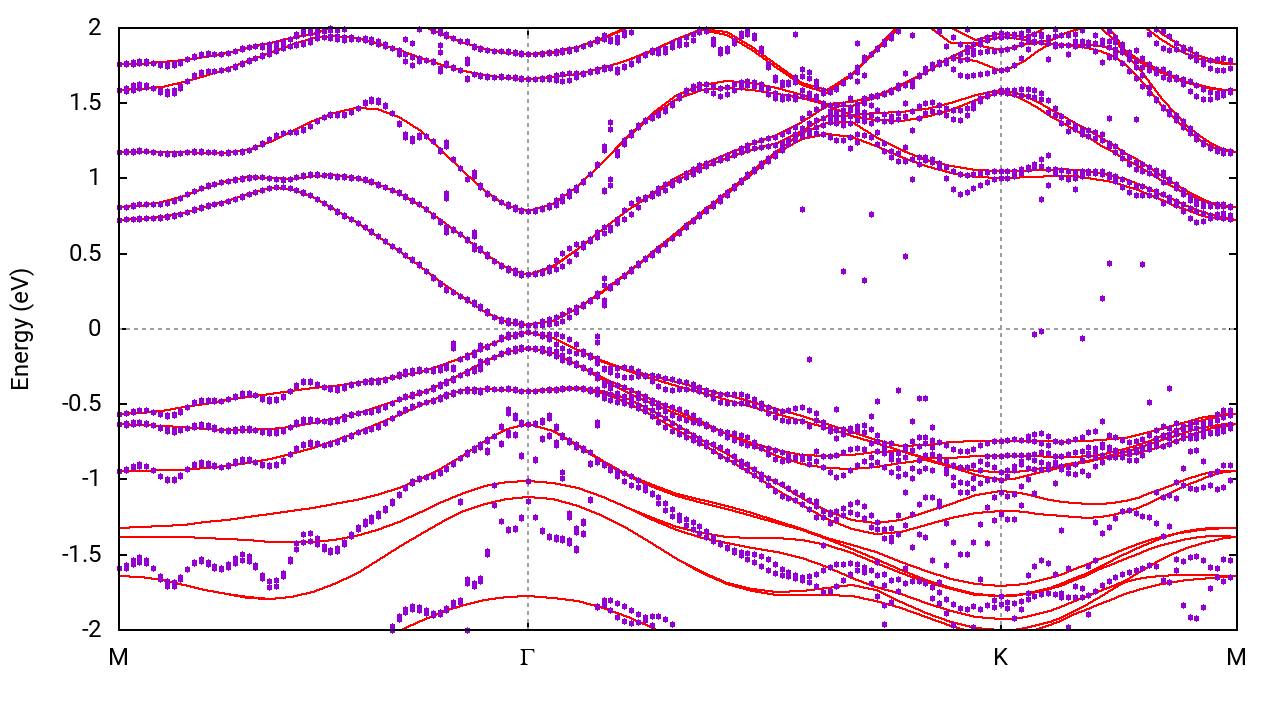
\includegraphics[width=\textwidth]{figure/Band_-1-0_to_3-0.png}\caption{{\small froz\_win:\([-1.0,3.0]\)}}
      \end{subfigure}
      \begin{subfigure}{0.42\textwidth}
         \centering
         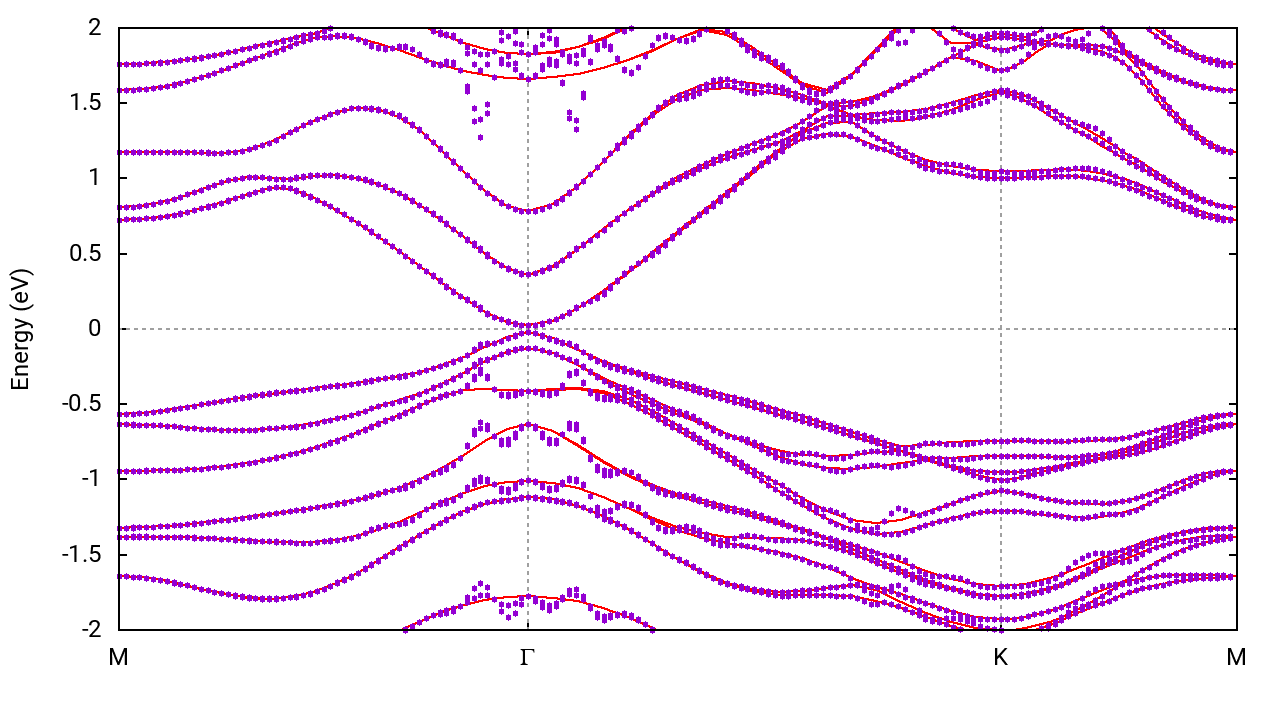
\includegraphics[width=\textwidth]{figure/Band_-2-0_to_2-0.png}
         \caption{{\small froz\_win:\([-2.0,2.0]\)}}
      \end{subfigure}
      \begin{subfigure}{0.42\textwidth}
         \centering
         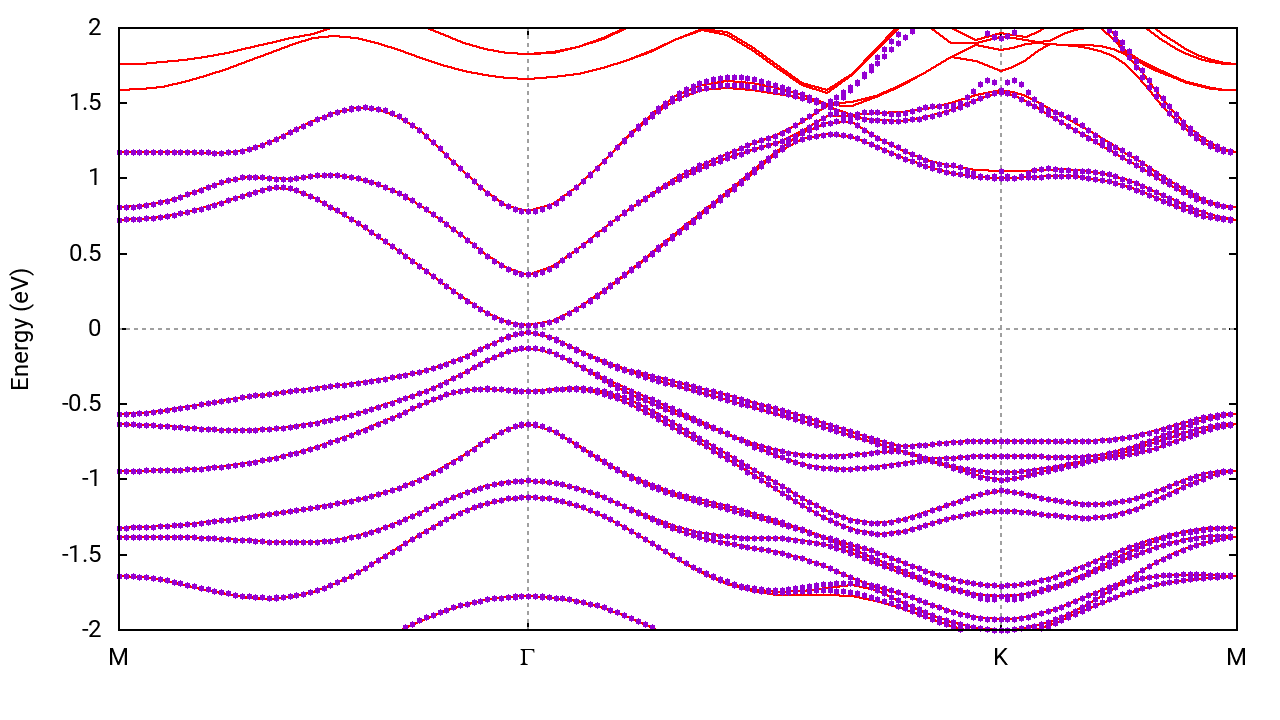
\includegraphics[width=\textwidth]{figure/Band_-1-5_to_1-5.png}
         \caption{{\small froz\_win:\([-1.5,1.5]\)}}
      \end{subfigure}
      \begin{subfigure}{0.42\textwidth}
         \centering
         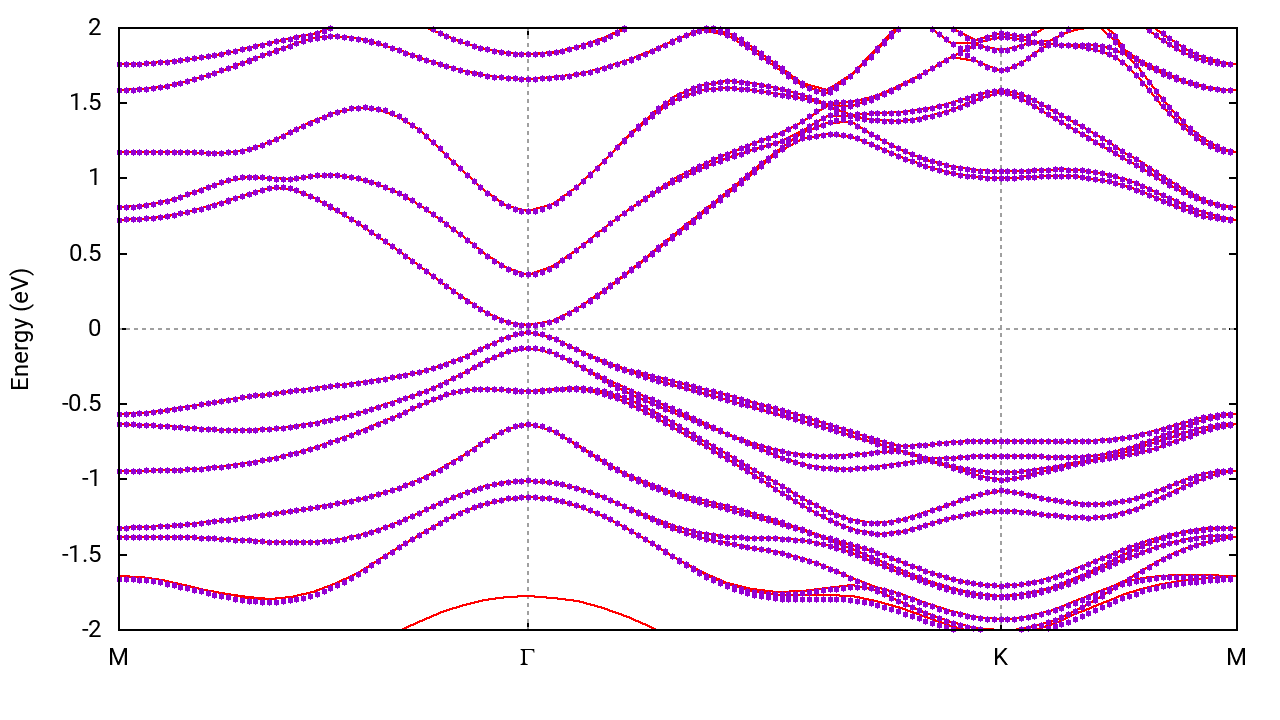
\includegraphics[width=\textwidth]{figure/Band_-1-5_to_2-0.png}
         \caption{{\small froz\_win:\([-1.5,2.0]\)}}
      \end{subfigure}
        \caption{Bands Calc. by VASP and \emph{Wannier90}}
    \end{figure}

  \end{frame}
  %%%%%%%%%%%%%%%%%%%%%%%%%%%%%%%%%%%%%%%%%%%%%%%%%%%%%%%%%%%%%%%%% 

  %%%%%%%%%%%%%%%%%%%%%%%%%%%%%%%%%%%%%%%%%%%%%%%%%%%%%%%%%%%%%%%%%
  \begin{frame}[fragile]
    \frametitle{Truth for WF Fitting}
    \begin{block}{As The Cow Say:}
      \begin{verbatim}

        ________________________________________
       / The truth is: wannier bands fitting is \
       \ a metaphysical problem.                /
        ----------------------------------------
               \   ^__^
                \  (oo)\_______
                   (__)\       )\/\
                       ||----w |
                       ||     ||
     \end{verbatim}
    \end{block}
  \end{frame}
  %%%%%%%%%%%%%%%%%%%%%%%%%%%%%%%%%%%%%%%%%%%%%%%%%%%%%%%%%%%%%%%%% 

  \section{Summary}

  %%%%%%%%%%%%%%%%%%%%%%%%%%%%%%%%%%%%%%%%%%%%%%%%%%%%%%%%%%%%%%%%%
  \begin{frame}
    \frametitle{Summary}
    \begin{block}{Summary}
      \begin{itemize}
        \item \textcolor{purple}{Wannier functions are Fourier transforms of the Bloch eigenstate.}
        \item Wannier functions are not uniquely defined.
        \item \textcolor{purple}{``Maximally Localized'' Wannier Function (MLWF) is one simple solution for constructing a well performed Wannier functions.}
        \item The process of obtain MLWF can be divided into two steps: optimize subspace, after which, optimize inside each fixed subspace.
        \item \textcolor{purple}{\emph{Wannier90} is a widely used Wannier fitting package.}
        \item Wannier fitting need a lot of experiment and, sometimes, is kind of tricky. 
      \end{itemize}
    \end{block}

  \end{frame}
  %%%%%%%%%%%%%%%%%%%%%%%%%%%%%%%%%%%%%%%%%%%%%%%%%%%%%%%%%%%%%%%%% 

  %%%%%%%%%%%%%%%%%%%%%%%%%%%%%%%%%%%%%%%%%%%%%%%%%%%%%%%%%%%%%%%%%
  \begin{frame}[fragile]
    \frametitle{Open Source Declaration}
    \large
    \begin{block}{Declaration}
      This slides is completely open-source, and protected by \textcolor{purple}{GPL3.0}. You can share or modify it based on any noncommercial purpose.\\[5pt]

      The source code and references are available on related \textbf{GitHub} repository:
      
      \textcolor{purple}{\url{https://github.com/kYangLi/PublicPresentation/tree/master/WannierFunctions}}
    \end{block}
    \tiny
    \begin{verbatim}
                                         __________________
                                        < Have a nice day! >
                                         ------------------
                                              \   ^__^
                                               \  (oo)\_______
                                                  (__)\       )\/\
                                                      ||----w |
                                                      ||     || 
    \end{verbatim}
  \end{frame}
  %%%%%%%%%%%%%%%%%%%%%%%%%%%%%%%%%%%%%%%%%%%%%%%%%%%%%%%%%%%%%%%%% 

\end{document}